\documentclass[tikz]{standalone}

\usepackage{anyfontsize}
\renewcommand{\normalsize}{\fontsize{16pt}{18pt}\selectfont}

\begin{document}
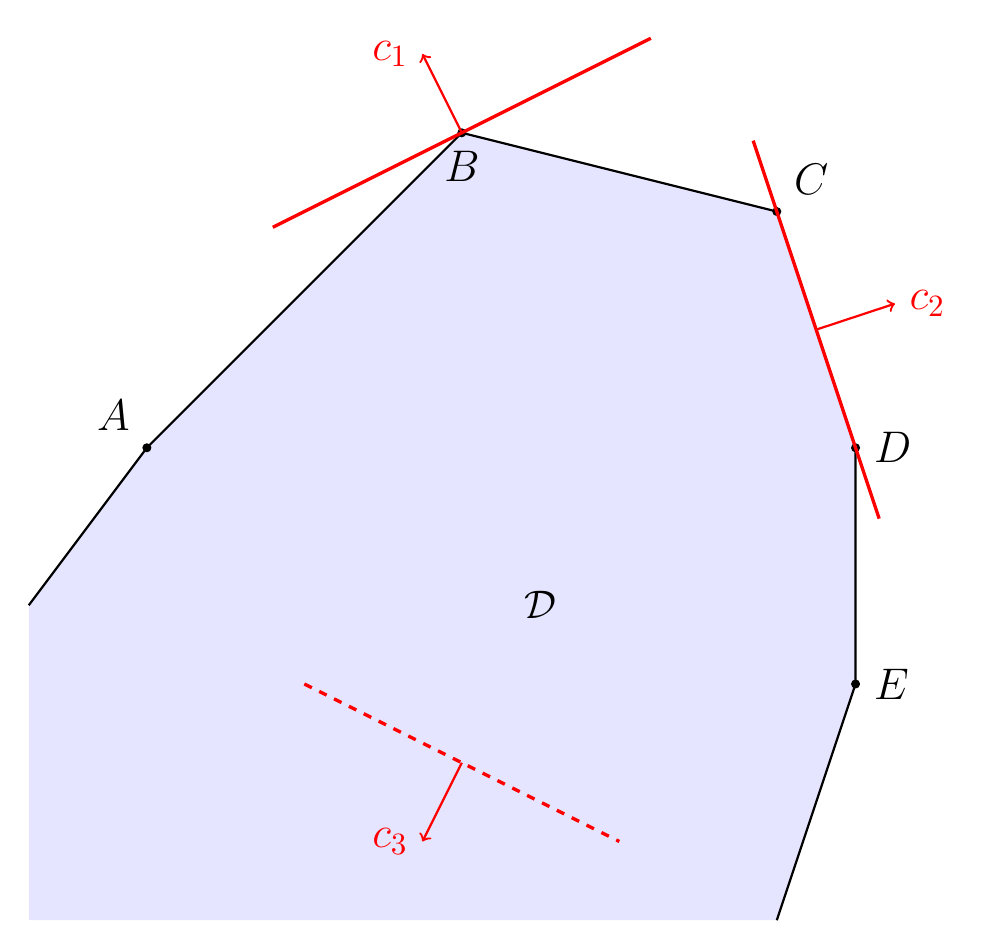
\begin{tikzpicture}[scale=1]

  % Define the two ray directions
  \coordinate (A) at (-5,2);
  \coordinate (B) at (-1,6);
  \coordinate (C) at (3,5);
  \coordinate (D) at (4,2);
  \coordinate (E) at (4,-1);

  % Prolong the rays to reach far down (e.g. y = -5)
  \path (A) -- ++(-1.5,-2) coordinate (Aext); 
  \path (E) -- ++(-1,-3) coordinate (Eext); 
  \coordinate (O) at (-6.5,-4);

  % Fill region defined by polygon and rays
  \fill[blue!10] (Aext) -- (A) -- (B) -- (C) -- (D) -- (E) -- (Eext) -- (O) -- cycle;

  % Draw polygon edges
  \draw[thick] (A) -- (B) -- (C) -- (D) -- (E);

  % Draw vertices.
  \node[draw,fill,circle,inner sep=1pt,label=above left:$A$] at (A) {};
  \node[draw,fill,circle,inner sep=1pt,label=below:$B$] at (B) {};
  \node[draw,fill,circle,inner sep=1pt,label=above right:$C$] at (C) {};
  \node[draw,fill,circle,inner sep=1pt,label=right:$D$] at (D) {};
  \node[draw,fill,circle,inner sep=1pt,label=right:$E$] at (E) {};

  % Draw the rays
  \draw[thick,black] (A) -- (Aext);
  \draw[thick,black] (E) -- (Eext);

  \node at (0,0) {\Large $\mathcal D$};

  % Draw LPs.
  \draw[red,very thick] (B)++(-2.4,-1.2) -- ++(4.8,2.4);
  \draw[red,->,thick] (B) -- ++(-0.5,1) node[left] {$c_1$};

  \draw[red,very thick] (C)++(-0.3,0.9) -- (D) -- ++(0.3,-0.9);
  \draw[red,->,thick] (3.5,3.5) -- ++(1,0.33) node[right] {$c_2$};

  \draw[red,very thick,dashed] (-3,-1) -- (1,-3);
  \draw[red,->,thick] (-1,-2) -- ++(-0.5,-1) node[left] {$c_3$};

\end{tikzpicture}
\end{document}
